\documentclass[../main.tex]{subfiles}

\begin{document}

\section{Use Case Description}
\label{section:problem:use_case}

\begin{figure}[h]
    \centering
    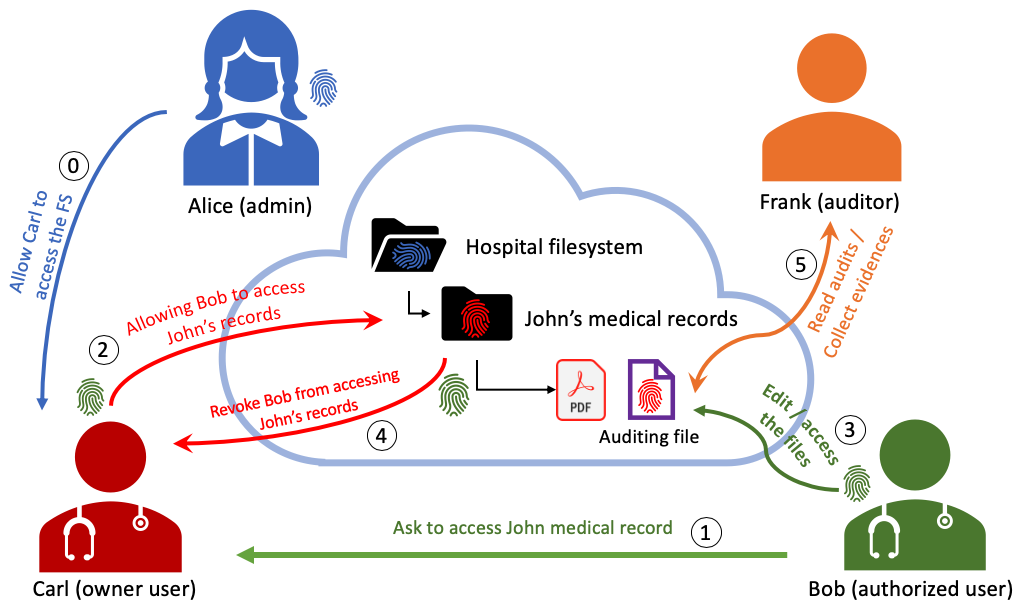
\includegraphics[width=0.75\textwidth]{../../images/problem/use_case}
    
    \caption{Use case representation}
    \label{figure:problem:use_case}
\end{figure}

\par Before going deeper into the protocol description we will first take a look at a higher level use case presented in Figure \ref{figure:problem:use_case}. First of all, we see that the resource shared between parties is what we call a filesystem. Furthermore, we see that three parties are intervening, each of them having a specific role. To explain each role, we are going to look at the scenario and explain one step at a time what is its purpose and who are the actors.

\par At first, we have Bob, the authorised user who needs to access a specific file or folder of the filesystem, John's medical record in this case. To do so, Bob must first be authorised by the owner user, Carl (e.g: Bob is a specialised doctor with an appointment with John and Carl is John's general practitioner). Carl will allow Bob to access this directory by linking Bob's fingerprint (the green fingerprint in Figure \ref{figure:problem:use_case}) to the target. In this way, Bob can now access the target when representing its fingerprint. Note that this process must be done online, every following action can then be freely done offline (at the condition of having a downloaded version of the Filesystem)
\par The very same process happens between Alice and Carl beforehand. The role of the administrator (Alice) is to create the filesystem and upload it to the cloud storage. She is also responsible for the user management: registering and assigning specific roles to each user. Note that, the administrator only deals with which user can access the Filesystem while the owner user decides which authorised user access which file or folder inside the Filesystem.
\par Once allowed, Bob can do whatever required actions he wishes (in the range set by Carl) at the condition that he specifies the purposes of each of them (e.g: this prevents Bob from accessing John's record outside an appointment and avoid Bob from abusing John's private information). Those intent are stored in an auditing file linked to each accessed file within the target directory. When Bob no longer needs to access John's records, Carl can simply remove its fingerprint from the target folder thereby preventing Bob to access newer versions of this directory.
\par Lastly, in the case of a GDPR inspection, an auditor, Frank, can retrieve and analyse the auditing files linked to John's records. Theses auditing files list all the operations made by users to a file, along with contextual information like the justification, the date/time and so on.

\end{document} 